\subsection{Results}
\todo[inline]{Chainge for EWSM}

We simulated two systems to evaluate the algorithms in four different configurations (See Figure \ref{fig:system-types}). The \simulationSimple{}{} system had equal weighting for each of the CTV components $\alpha, \beta, \gamma$. Each of the $13$ nodes was able to connect to $3$ other nodes to allocate measurement tasks. The sink node was given $5$ measurement tasks, with each node being able to perform these tasks with increasing quality dependant on their closeness to the demand point associated with the task. $3$ sets of the same measurement tasks were given to the same sink node before one episode was complete and the batteries of all nodes in the system was allowed to recharge fully (Figure\ref{fig:balanced_simulation}). 

The \simulationExtended{}{} system had CTV component weighting where each of the relevant properties were given an $80\%$ dominance over the value of CTV value. The sink node was given $10$ measurements to allocate, with no repetition. It was also placed at a significantly large distance from the demand points associated with the tasks, which the other $25$ nodes in the system could then receive and allocate or execute. This system gave a contrasting choice between allocating tasks in such a way that task value could be maximised, but at the cost of longer arcs and therefore energy usage, or lower task values, and lower energy consumption. This allowed the comparison of the learning algorithms given different CTV weightings (Figure\ref{fig:unbalanced_simulation})

\begin{figure}[ht]
	\centering
	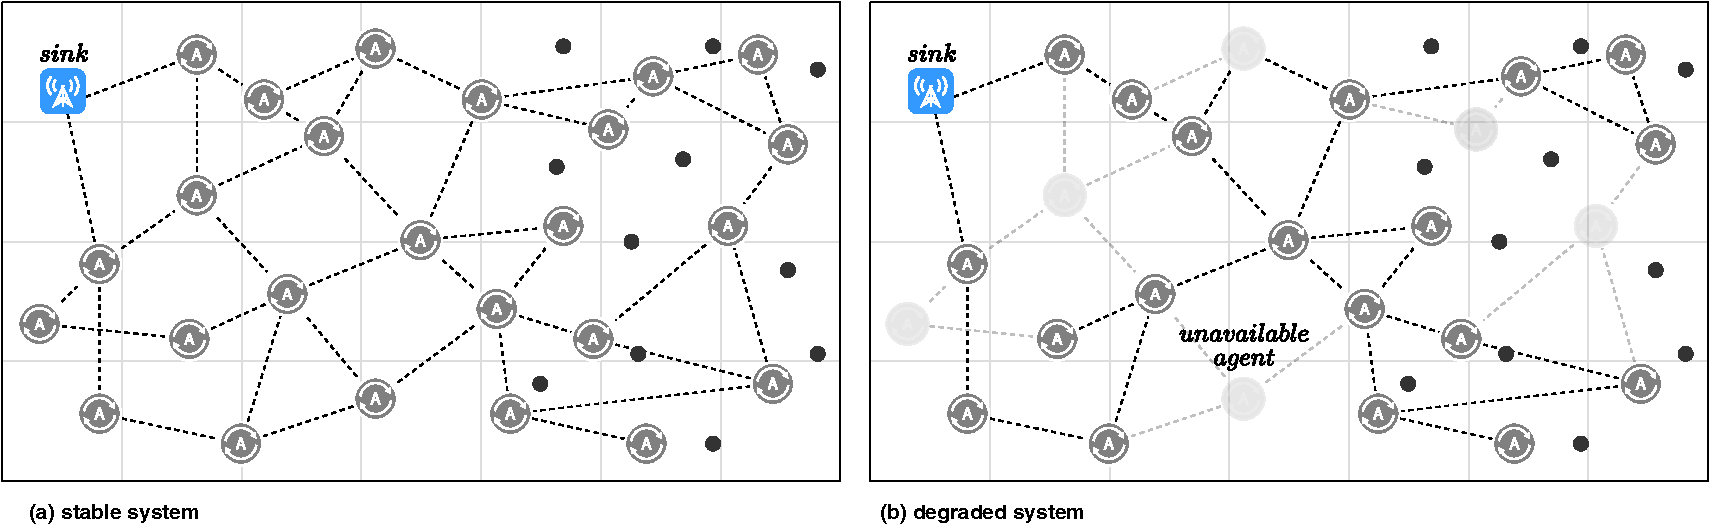
\includegraphics[width=0.9\linewidth]{system-types}
	\caption{\textbf{System types}. The diagram shows examples of the two systems. In the first \simulationSimple{}{}, there are $10$ possible agents that can execute the measurement task, tasks' demand points are distributed across the map. In the second, \simulationExtended{}{} system, there are $25$ agents that can execute the measurement tasks. The tasks' demand points are clustered away from the sink node.}
	\label{fig:system-types}
\end{figure}

Labels and descriptions for the algorithms are shown in Table \ref{table:summary_of_algorithms}, with configuration in Table \ref{table:summary_of_configurations}. Results for the \algorithmBalanced{}{} algorithm in the \simulationSimple{}{} system, and the \algorithmEnergy{}{}, \algorithmQuality{}{}, \algorithmDistribution{}{} algorithms in the \simulationExtended{}{} system are shown in Tables \ref{table:results_balanced} and \ref{table:results_unbalanced} respectively.
\todo[inline]{explain the results table and graph comparisons here}

Figure XXX shows the 